\section{Discussion and Conclusion}\label{sec:conclusion}

We have measured the local PNG parameter $\fnl$ using the scale-dependent bias in the angular clustering of LRGs selected from the DESI Legacy Imaging Survey DR9. Our sample includes more than $12$ million LRG targets covering around $14,000$ square degrees in the redshift range of $0.2< z < 1.35$. We leverage early spectroscopy during DESI Survey Validation \citep{desi2023sv} to infer the redshift distribution of our sample (Figure \ref{fig:nz}). \mr{Our power spectrum model accounts for various theoretical and observational effects such as RSD, magnification bias, survey geometry, and integral constraint. Most importantly, we utilize a novel machine learning-method to mitigate the effect of imaging systematics and reduce excess clustering power on large scales (or low $\ell$).}

In our fiducial analysis, \mr{which includes a non-linear treatment of systematics using nine imaging property maps (Galactic extinction, stellar density, depth in $grzW1$, and psfsize in $grz$), we obtain $\fnl = 34^{+24(+50)}_{-44(-73)}$ with $p=1$ and $s=0.945$. This measurement is consistent with recent CMB and LSS measurements, as visualized in Figure \ref{fig:fnlhist}. The sensitivity of our constraints is explored against $p$ and $s$. Specifically, we find that the error on $\fnl$ is more sensitive to $p$ than $s$. Compared with the fiducial result, the error increases by more than a factor of two for $p=1.6$, and only by $7\%$ for $s=1.25$ (Figure \ref{fig:fnl_magbias}). The minimum $\chi^{2}$ however does not change much, indicating that the impact on the power spectrum fit is negligible.} 

\mr{The signature of local PNG is very sensitive to excess clustering power caused by imaging systematic effects. We have applied a series of robustness tests to investigate the impact of how the galaxy selection function is determined. Specifically, both linear and nonlinear methods are applied using various combinations of imaging systematic maps (including two external maps for the neutral hydrogen column density and photometric calibration error in the z band). We also examine the effect of additional masks based on imaging conditions and survey completeness. Overall, we find no change in the analysis that shifts the maximum likelihood value of $\fnl$ to a significantly different value (Figure \ref{fig:mcmc_dr9reg}, Figure \ref{fig:mcmc_dr9elmin}, and Table \ref{tab:dr9method}).}

\begin{figure}
    \centering
    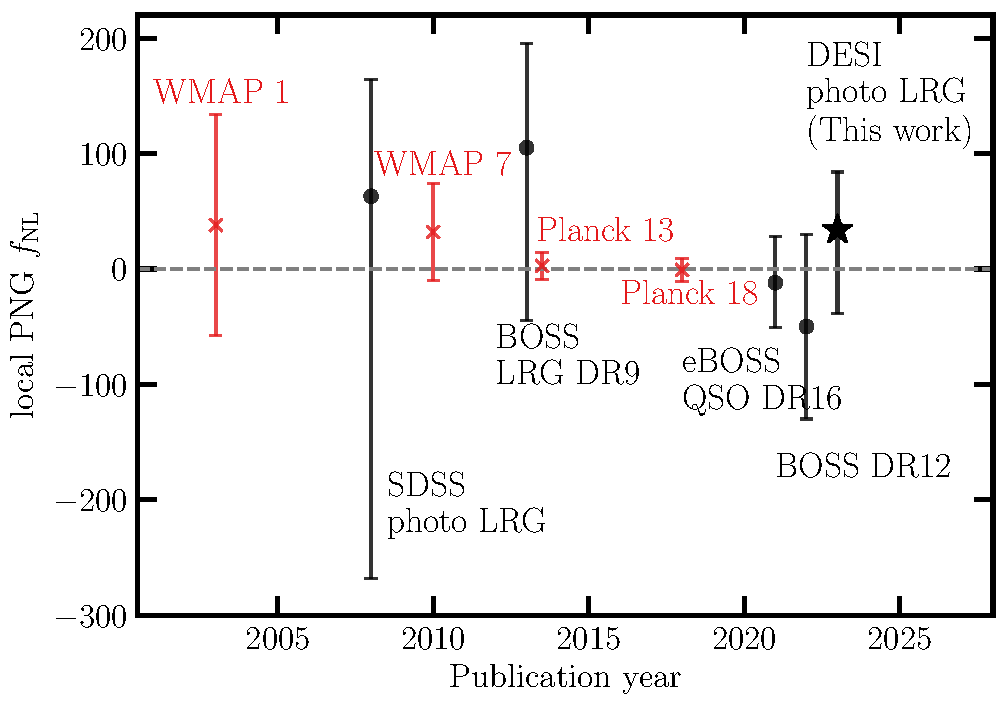
\includegraphics[width=0.45\textwidth]{figures/fnl_history.pdf}
    \caption{History of constraints on local PNG $\fnl$ at $95\%$ confidence from single-tracer LSS \citep{slosar2008constraints,2013MNRAS.428.1116R, mueller2022primordial, 2022PhRvD.106d3506C}, including our analysis with $\mr{-39}<\fnl<\mr{84}$ (DESI photo LRG) and CMB surveys \citep{Komatsu_2003, Komatsu_2010, planck13, akrami2019planck}. The median $\fnl$ value is used in case the maximum likelihood estimate was not reported in the reference.}
    \label{fig:fnlhist}
\end{figure}

\mr{Although being essential for the mitigation of imaging systematics, the template-based approach inevitably removes some of the large-scale clustering information. One of the primary highlights of this work is that we present a strategy to calibrate the systematic mitigation's impact on the inferred $\fnl$. As we increase the number of maps for mitigation, more of the power spectrum is removed, introducing a larger bias to the $\fnl$ posterior distribution. Our mock tests suggest that this bias is $\fnl$-dependent, such that the mocks with larger $\fnl$ experience a more substantial reduction in the low$-\ell$ power due to systematic mitigation.}

\mr{We conduct regressions using a smaller set of maps, including Galactic extinction, depth in the z band, and astronomical seeing in the r band (nonlinear three maps) to retain some constraining power. Additionally, we consider an additional map for local stellar density (nonlinear four maps). Using three or four maps, we can qualitatively mitigate systematic trends in the mean galaxy density and cross correlations of the galaxy density field and imaging property maps (see Appendix \ref{sec:systests}). With these methods, the error on $\fnl$ does not degrade as much as the fiducial method. However, we realize that a quantitative assessment of these residual systematics depends on covariance matrices and, notably, the $\fnl$ value used for creating the mocks. Therefore, our findings underscore the importance of exploring, developing, and validating alternative mitigation approaches to avoid over-correction for a robust analysis of local PNG.}

Our analysis can be considered as the first attempt to identify major systematics in DESI, so we can be ready for constraining $\fnl$ with DESI spectroscopy. Internal DESI tests of the photometric calibration were unable to uncover DESI-specific issues, e.g., when comparing to Gaia data. The most significant trends that we find are with the E(B-V) map. The source of such a trend would be a mis-calibration of the E(B-V) map itself or the coefficients applied to obtain Galactic extinction corrected photometry. Such a mis-calibration would plausibly be proportional in amplitude to the estimated E(B-V) map, though it may not have E(B-V)’s spatial distribution. \mr{In order to explain the excess signal we measure using nonlinear three maps or nonlinear four maps, such an effect would need to be approximately twice that of the trend we find with E(B-V)}. There are ongoing efforts within DESI to obtain improved Galactic extinction information, which will help establish if this is indeed the cause. \mr{Additionally, cross-correlations of the DESI LRG density with the CMB lensing map is more stable in terms of systematics and can complement the results presented in this work. Additionally, we can further avoid the over-fitting issue by combining our neural network-based treatment method with forward-modeling techniques, such as Obiwon \citep{kong2020}, but we will leave that for future work.} 
